For each of Problems~\ref{p:1}-\ref{p:3}, extensive experimental evaluations were carried out to evaluate our proposed algorithmic solutions. Here, we present representative evaluation demonstrating the effectiveness of our methods, with a focus on three realistic settings (the ICU model from Fig.~\ref{fig:ex}, bus and subway car models shown in Fig.~\ref{fig:bus-subway}). %
For all environments, the surface $S$ is selected to be all visible surfaces not facing downward.
Due to limited space, result on the (2+$\varepsilon$)-approximation algorithm (Algorithm~\ref{alg:greedy}) is omitted (as shown in \cite{FenYuRSS20}, such methods are fast but are quite sub-optimal). The experiments were carried out on a median-end quad-core Intel i7 processor with 16GiB RAM. 
Algorithms were implemented in C++. Gurobi \cite{gurobi} was used as the Integer Programming solver. 
Source code is available at 
{\small \url{https://github.com/rutgers-arc-lab/3d_coverage}}.

\begin{figure}[!ht]
    \centering
    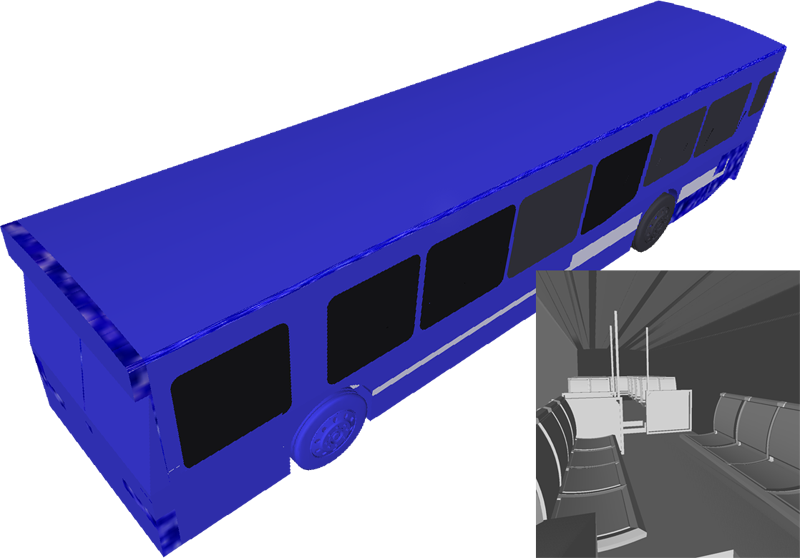
\includegraphics[width = .4\columnwidth]{chapters/surf/fig/bus.png}\hspace{3mm}
    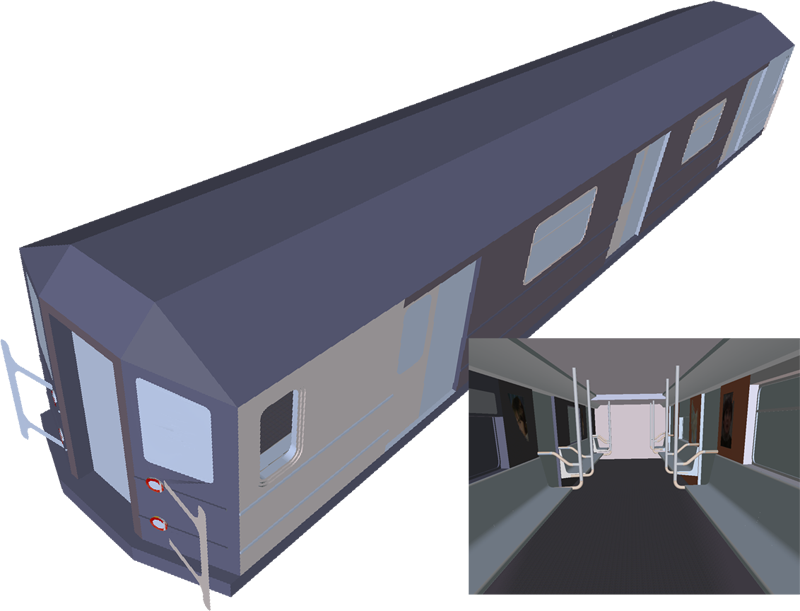
\includegraphics[width = .4\columnwidth]{chapters/surf/fig/subway.png}
    \caption{Realistic 3D environments used in our evaluation in addition to the ICU model from Fig.~\ref{fig:ex}. [left] A 40-foot large bus model and its interior. [right] A subway car and its interior.}
    \label{fig:bus-subway}
\end{figure}

Results on Problem~\ref{p:1}, using ILP, is given in Fig.~\ref{fig:coverage-ratio-vis}. 
For each model, $600$ candidate sensor locations and $20,000$ coverage surface points are sampled using grids. 
As expected, the surface coverage ratios increase as the number of sensors increase, approaching full coverage. We note that certain surface region is not visible, e.g., ground underneath seats in subway cars, leading to plateaus below $100\%$ coverage. The computation time is very reasonable for offline computations. The spikes in the middle of the computation time plot correspond to hard cases when the visibility coverage is about to plateau. We also observe that subway $<$ ICU $<$ bus in terms 
of computation time, which may be explained by the interior complexity of these environments. This aspect is different across the three problems.

\begin{figure}[!ht]
\vspace{1mm}
    \centering
    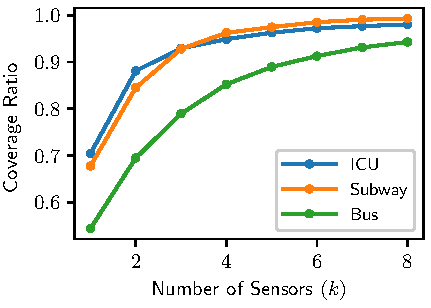
\includegraphics[width=0.475\columnwidth, height=1.in]{chapters/surf/fig/result-coverage-ratio-eps-converted-to.pdf}
    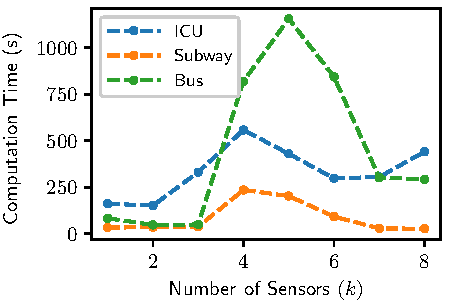
\includegraphics[width=0.49\columnwidth,height=1.in]{chapters/surf/fig/result-time-eps-converted-to.pdf}
    \caption{Coverage quality and computation time for Problem~\ref{p:1} for the three environments as the number of sensors change.}
    \label{fig:coverage-ratio-vis}

\end{figure}

\begin{wrapfigure}[7]{r}{1.1in}
  \vspace*{0mm}
  \begin{overpic}[width=1.1in,tics=5]{chapters/surf/fig/terrain-8.png}
	\end{overpic}
\vspace*{-6.5mm}
\end{wrapfigure}
In evaluating Problem~\ref{p:2}, we first examine a case where mobile sensors
(e.g., camera drones) are deployed to cover a synthetic terrain with relatively 
small curvature, i.e., $vis(\cdot, \cdot) \equiv 1$. An illustration of the 
setting is given in the figure on the right, where the color indicates the height 
of the terrain. The sensors (8 red triangles in the figure) are placed
at a fixed height above the terrain and must guard the region enclosed 
in the black curve. Spherical range sensing is assumed. For the setup 
($600$ sensor locations and $20,000$ surface points), computation time 
and solution quality as the number of sensors changes are listed in the table. Computation time decreases as the number of sensors 
increases, indicating the problem is harder when sensors are too few to provide 
a good coverage. It also shows that the ILP running time does not depend positively
on sensor quantity. The quality (smaller is better) increase becomes minimal
as sensor quantity reaches $10$. 


\vspace{1mm}
\begin{table}[!ht]
    \centering
    \begin{tabular}{|c|c|c|c|c|c|c|c|c|}
    \hline
        \#Sensors   & 2     &  4    & 6      & 8     & 10    & 12    & 14    & 16 \\
        \hline
        Time (s)    & 42.9   &  25.4    & 18.5  & 12.7 & 13.1  & 11.3  & 7.64 & 6.70 \\ 
        \hline
        Radius  & 5.10     &  3.31    & 2.76      & 2.43     & 2.27    & 2.16    & 2.07    & 1.99 \\
        \hline
    \end{tabular}
    %\caption{Computation time and minimum radius for the problem 2 without visibility issue computed on a randomly generated terrain.}
    \label{tab:Terrain}
\end{table}

In a second evaluation of Problem~\ref{p:2}, visibility is considered with the 
optimization coverage ratio set to $80\%$. That is, at least $80\%$ of the
maximum visible target surface (for a given $k$) will be guaranteed the achieved coverage 
quality. The result, summarized in Fig.~\ref{fig:coverage-ratio-mq}, again 
demonstrates a negative correlation between the computational time and the number 
of sensors. Here, however, the computational time is $20+$ times  more 
than when having full visibility.

\begin{figure}[!ht]
    \centering
    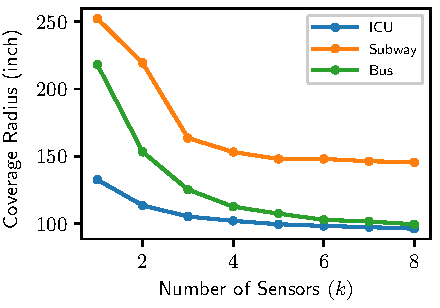
\includegraphics[width=.46\columnwidth, height=0.98in]{chapters/surf/fig/result-radius-mq-eps-converted-to.pdf}
    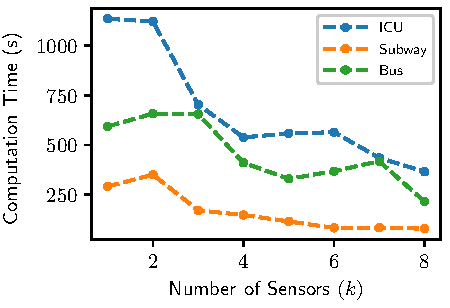
\includegraphics[width=.49\columnwidth, height=1.in]{chapters/surf/fig/result-time-mq-eps-converted-to.pdf}
    \caption{Coverage quality (lower is better) and computation time for Problem~\ref{p:2}
    for the three environments, as sensors increase.}
    \label{fig:coverage-ratio-mq}
\end{figure}

Our last benchmark on Problem~\ref{p:2} tests the effectiveness of the local improvement following the resolution of a coarsely generated ILP, at $60$ candidate sensor locations and $1000$ surface samples (Fig.~\ref{fig:coverage-ratio-cu}). The right figure shows much faster computation time. The left figure shows that the  faster method does a decent job for the bus environment (other environments have similar outcomes). The result suggests which method to use would depend on whether computational time or solution optimality is more important to the task at hand. We note that the local improvement method does not help improve the ILP result at the higher resolution. 

\begin{figure}[!ht]
    \centering
    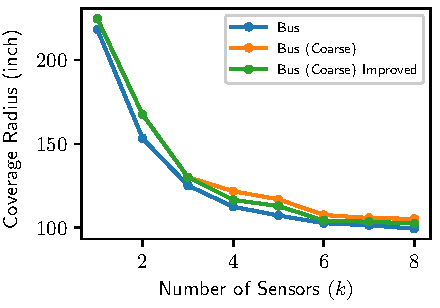
\includegraphics[width=.48\columnwidth, height=1.in]{chapters/surf/fig/result-bus-mq-eps-converted-to.pdf}
    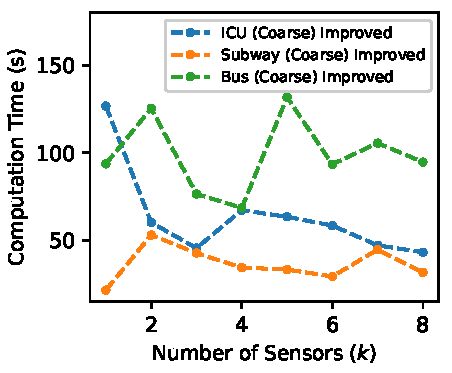
\includegraphics[width=.48\columnwidth, height=1.in]{chapters/surf/fig/result-time-mq-coarse-eps-converted-to.pdf}    
    \caption{ [left] Solution quality (lower is better) for the bus environment. 
    The first curve (Bus) is the same as that from Fig.~\ref{fig:coverage-ratio-mq}. 
    [right] Computation time using coarse ILP + local improvement.}
\label{fig:coverage-ratio-cu}
\end{figure}

For Problem~\ref{p:3}, computation becomes more demanding. At the specified 
discretization level, most ILP models did not complete the optimization process 
in $10$ minutes. The intermediate quality result is given in Fig.~\ref{fig:computation-time-3}, on the left (the same threshold, selected to make the computation challenging, is used for all three environments), where the lines 
corresponds to the coverage ratio returned by the ILP model and the attached vertical bars show the reported optimality gap. The crosses show the updated ratio after local improvement is carried out (the triangles will be explained shortly). 
The subway data was shifted to the left to improve readability.
For the bus, we see that the local improvement does help improve solution optimality, suggesting it is the most difficult problem. For the other two, it appears that the solution by the ILP model is already quite optimal, but the ILP solver still needs time to close the gap from the above. The subway case has worse coverage by the same number of sensors because it is larger. If we run a coarse ILP model ($60$ sensor candidates, $1000$ surface sample) for one minute and then do local improvement, we get coverage ratios shown as the triangles in Fig.~\ref{fig:computation-time-3}, left. Fig.~\ref{fig:computation-time-3}, right shows the total computation time used. We observe that except for the challenging bus model, the faster method achieves essentially identical optimality as running ILP at higher resolutions. Subway costs most time here because it is the largest. 

\begin{figure}[!ht]
    \centering
    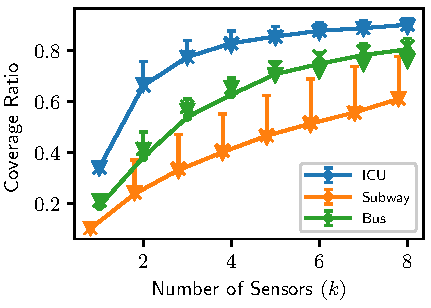
\includegraphics[width=.48\columnwidth, height=1in]{chapters/surf/fig/result-coverage-ratio-3-eps-converted-to.pdf}
    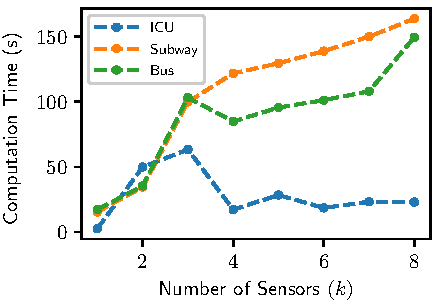
\includegraphics[width=.48\columnwidth, height=1in]{chapters/surf/fig/result-time-3-coarse-eps-converted-to.pdf}
    \caption{[left] Coverage ratio (lines) for Problem~\ref{p:3} returned by multiple methods. [right] Computation time used by running a coarse ILP plus local improvements.}
    \label{fig:computation-time-3}
\end{figure}

% For the last evaluation of Problem~\ref{p:3}, 

Lastly, we provide some additional visualization to help further demonstrate the structure of the problems. Fig.~\ref{fig:icu-comp} shows that Problems~\ref{p:2} and~\ref{p:3} induce different optimal distribution of sensors. Generally, Problems~\ref{p:2} tends to cause the sensors to be evenly spaced out. On the other hand, Problem~\ref{p:3} tends to balance between spacing out sensors and provide good cumulative coverage, which may require sensors to aggregate, which can be observed in Fig.~\ref{fig:bus}.

\begin{figure}[!ht]
\vspace{1mm}
    \centering
    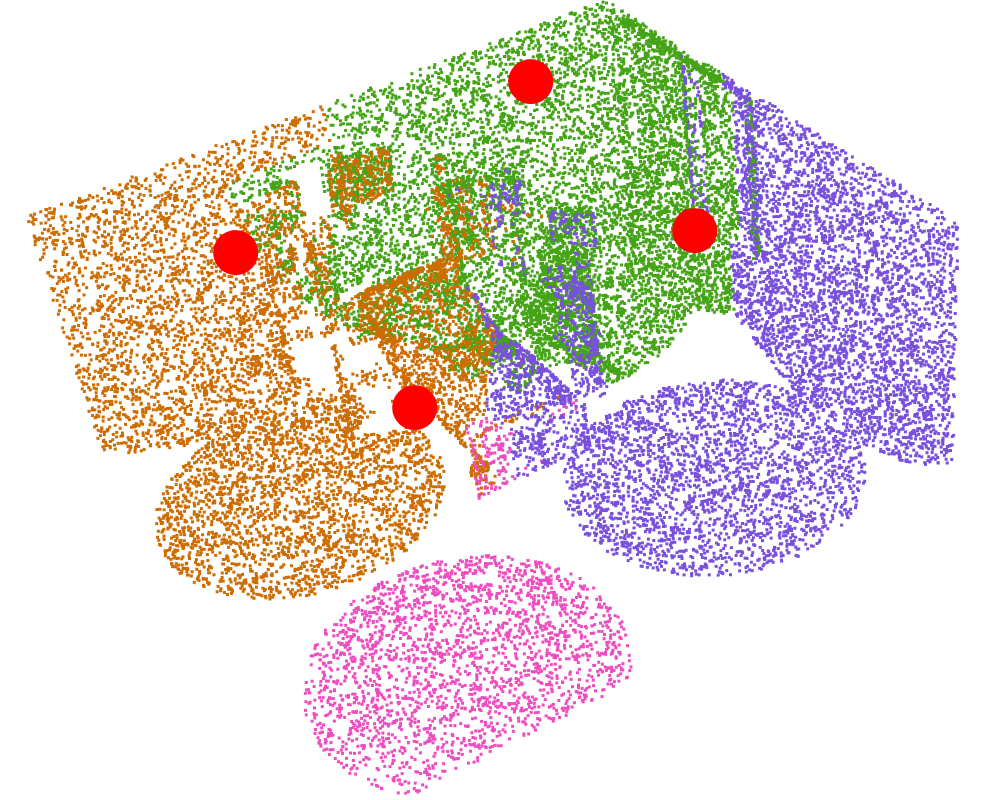
\includegraphics[width = 0.35\columnwidth]{chapters/surf/fig/icu-2-4.png}\hspace{3mm}
    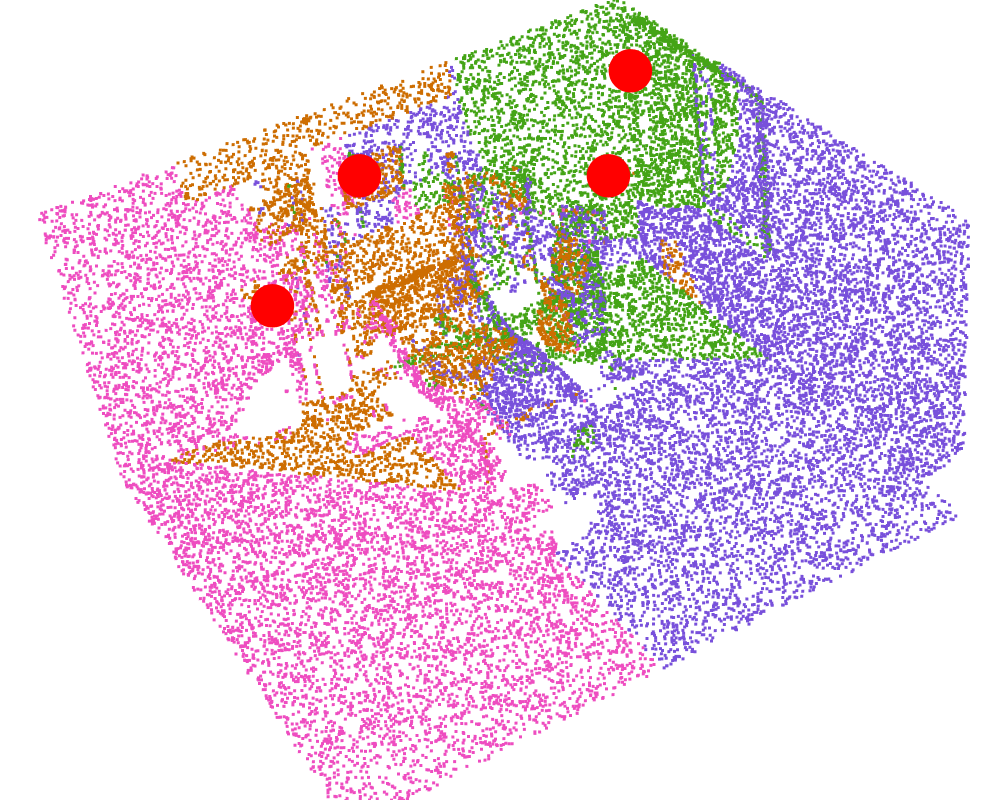
\includegraphics[width = 0.35\columnwidth]{chapters/surf/fig/icu-3-4.png}
\vspace{1mm}
    \caption{$4$ sensor ICU result for Problems~\ref{p:2} (left) and~\ref{p:3}(right).}
    \label{fig:icu-comp}
\end{figure}

\begin{figure}[!ht]
\vspace{-1mm}
    \centering
    \includegraphics[width = .25\columnwidth]{chapters/surf/fig/illustration_bus.png}
    %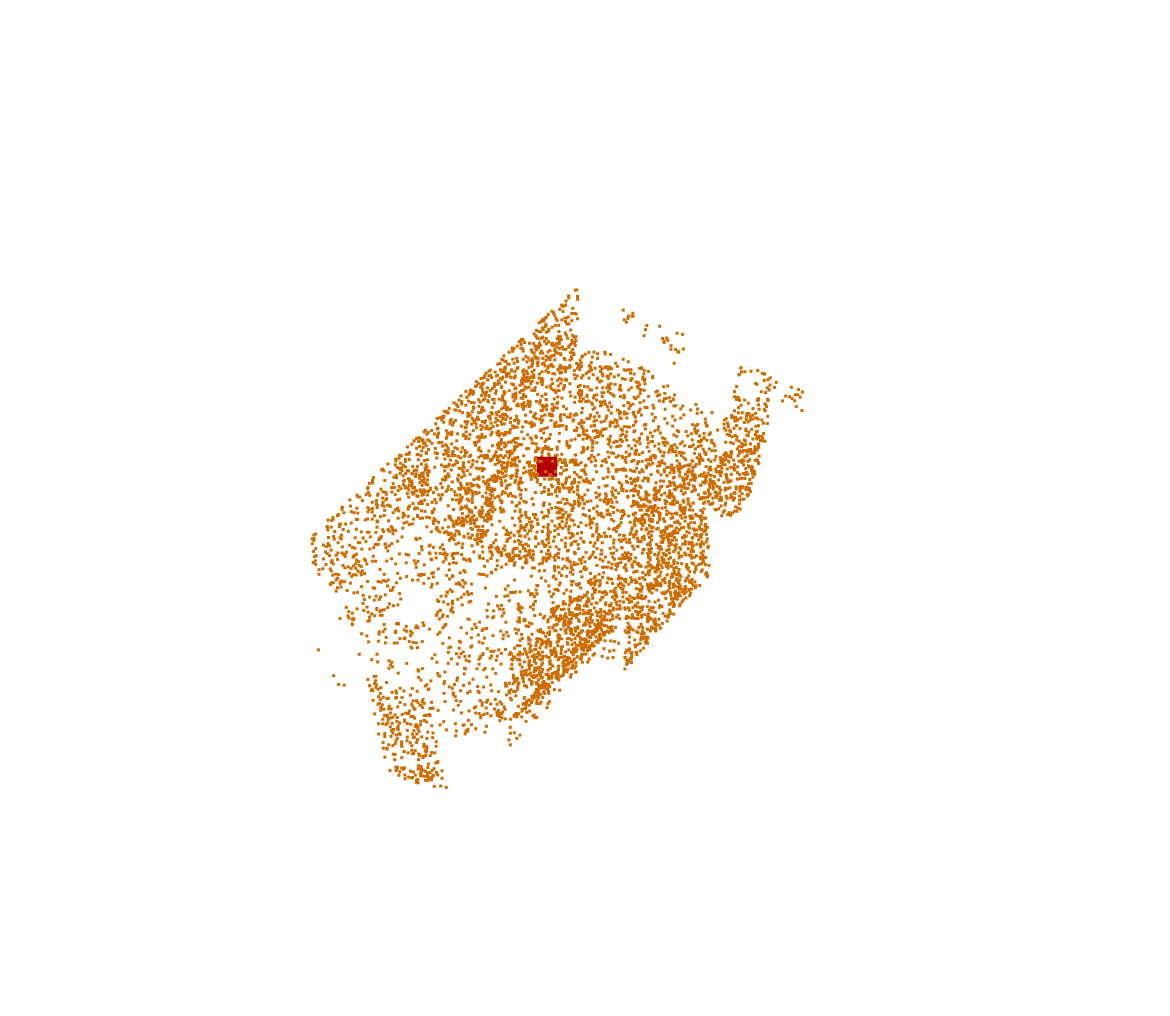
\includegraphics[width = .31\columnwidth]{fig/illustration_bus_1.png}
    %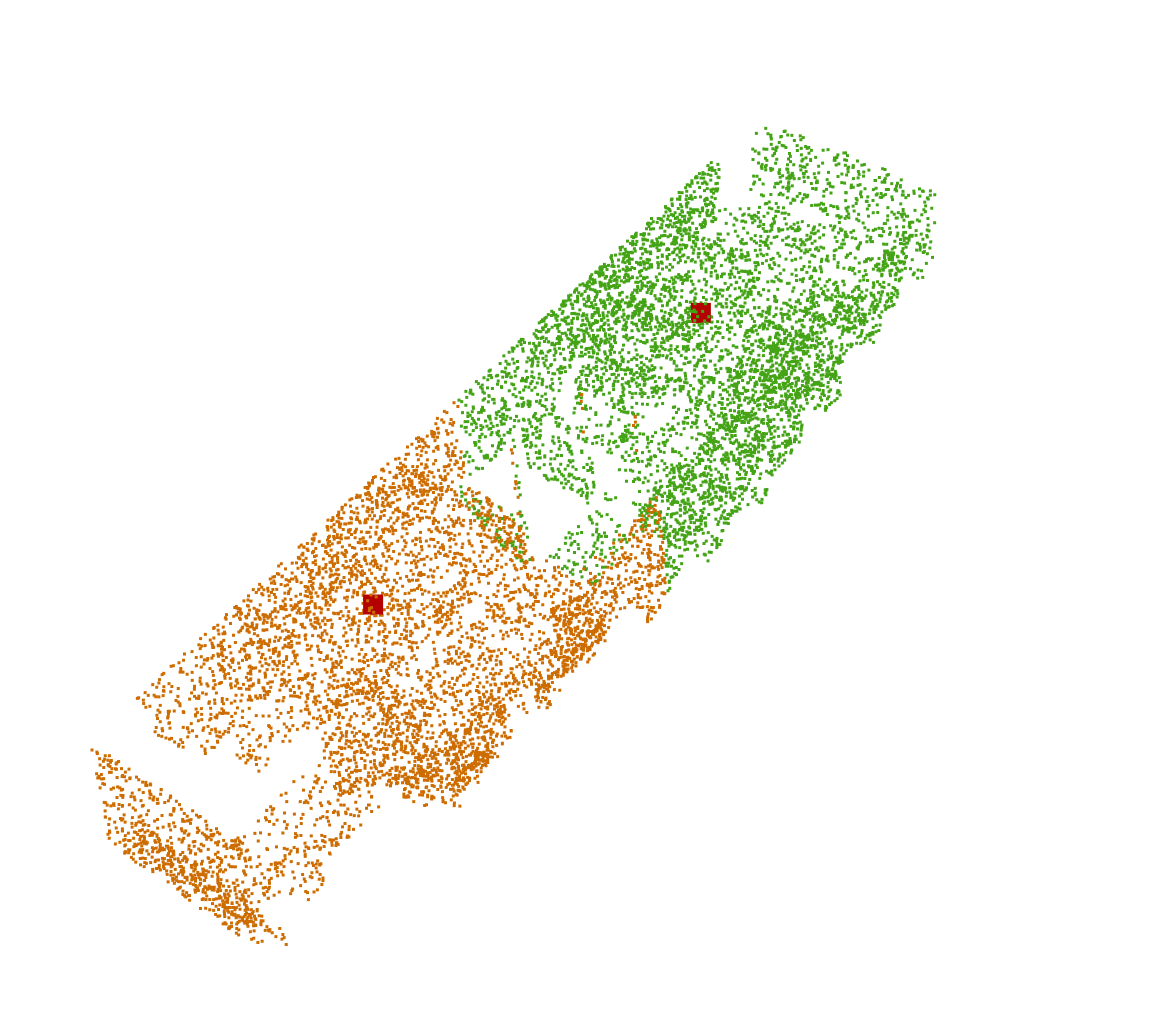
\includegraphics[width = .31\columnwidth]{fig/illustration_bus_2.png}
    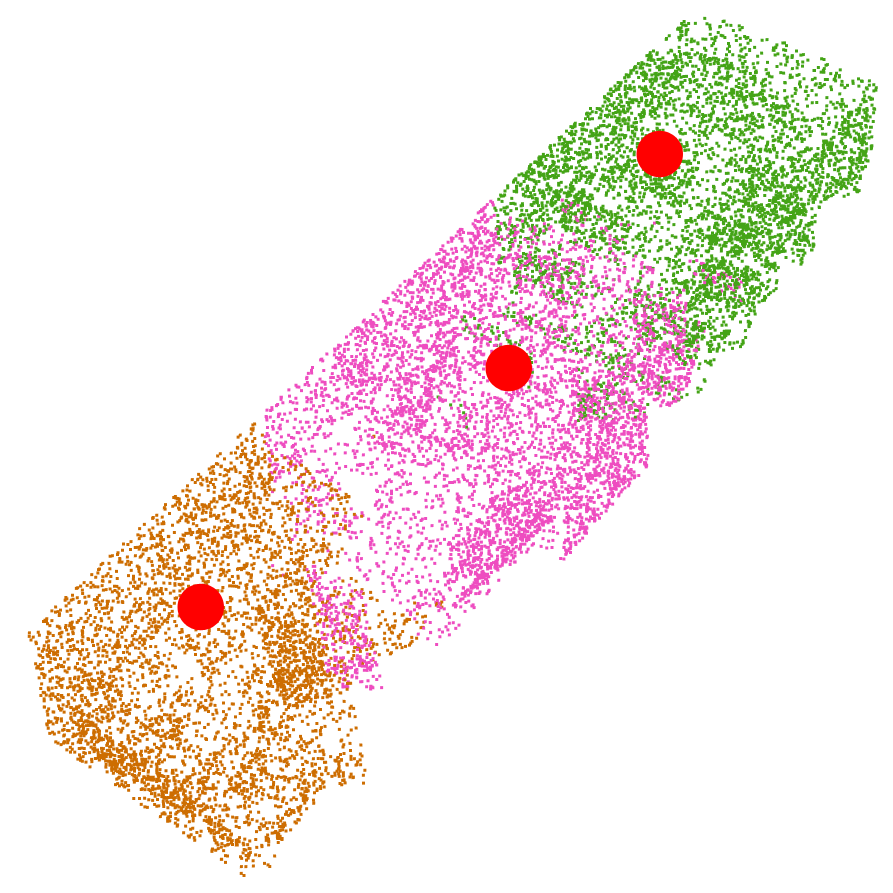
\includegraphics[width = .23\columnwidth]{chapters/surf/fig/bus-3-3.png}
    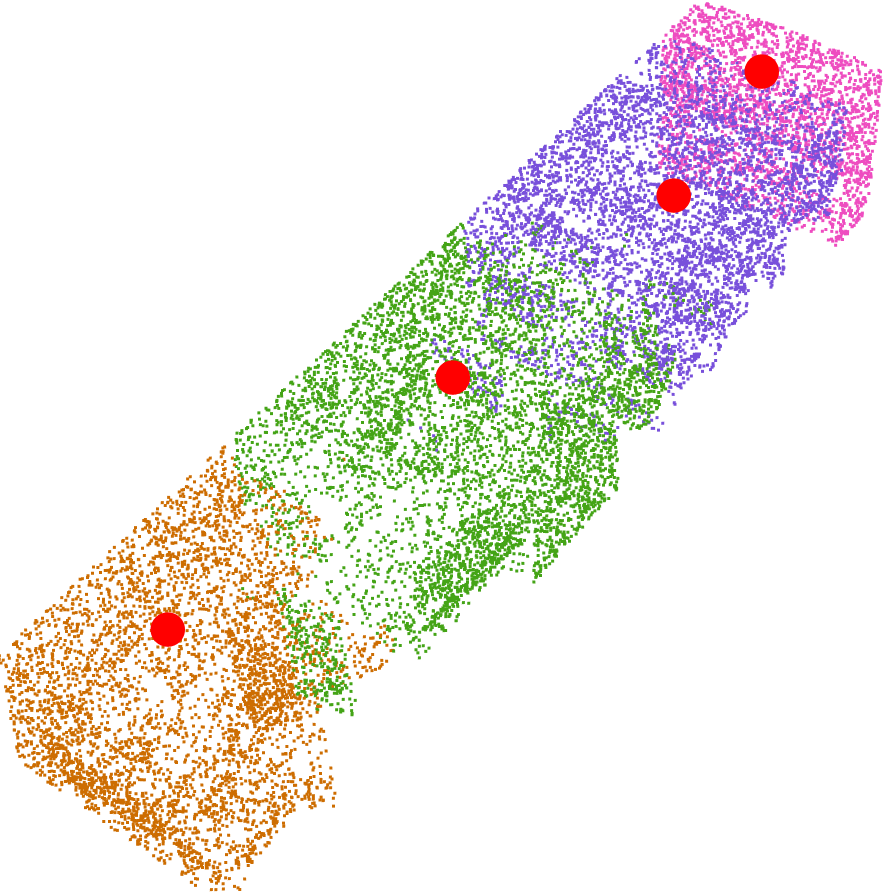
\includegraphics[width = .23\columnwidth]{chapters/surf/fig/bus-3-4.png}
    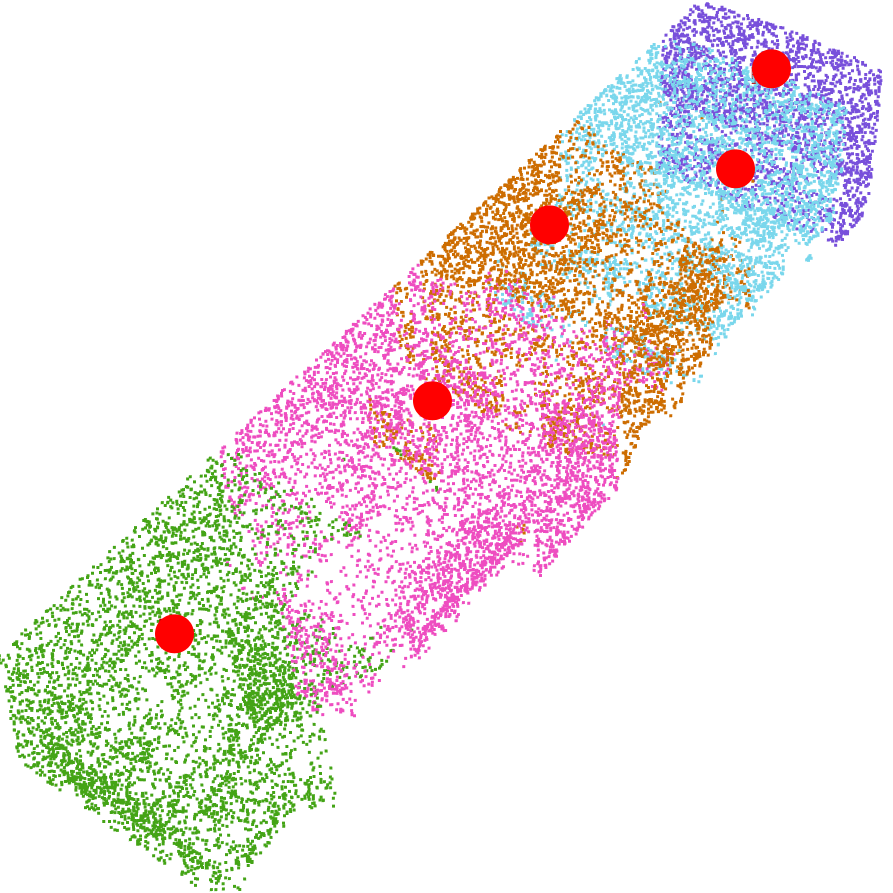
\includegraphics[width = .23\columnwidth]{chapters/surf/fig/bus-3-5.png}
    \caption{The coverage of bus (see through model on the left) using $3$ to $5$ sensors under Problem~\ref{p:3}. Aggregation of sensors at the front of the bus, which is structurally more complex, can be observed. }
    \label{fig:bus}
\end{figure}



%\begin{figure}[!ht]
%    \centering
%    \vspace{-0.5in}
%    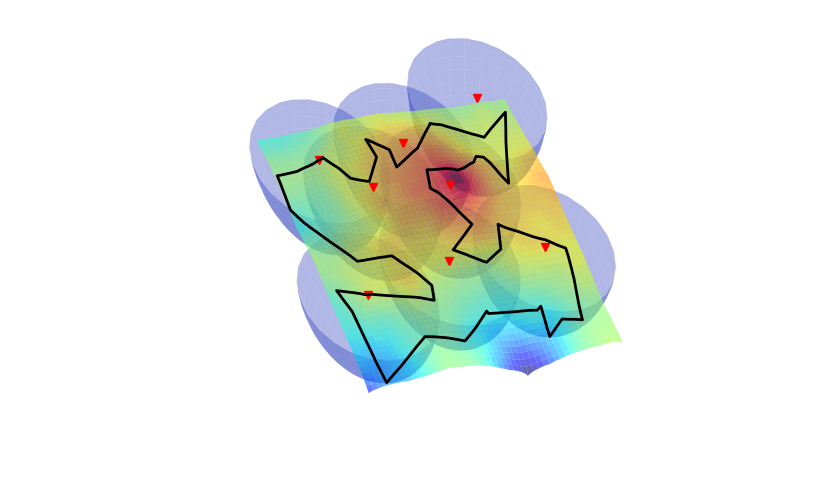
\includegraphics[width=\columnwidth, height=1.65in]{fig/terrain_8_spheres.png}
%    \vspace{-0.5in}
%    \caption{Covering a randomly generated terrain region (enclosed in black lines) with %8 sensors, for Problem~\ref{p:2}.}
%    \label{fig:terrain_8_spheres}
%\end{figure}

%% Coverage quality - # sensor curve for visibility model
% \begin{comment}
% Experiment data:
% Visibility:

% ICU computation time
% 161.070609 151.295530 330.685622 557.836444 429.295166 297.618731 304.730803 440.795053
% Coverage out of 20000
% 14082 17622 18588 18975 19252 19445 19535 19608

% Train computation time
% 33.274342 34.031417 37.465971 235.116101 202.418864 91.999594 28.336419 26.826848
% Coverage out of 20000
% 13549 16903 18557 19250 19492 19704 19811 19856

% Bus computation time
% 82.551965 47.326792 49.360691 819.235458 1155.414985 843.010299 301.578288 292.435206
% Coverage out of 20000
% 10874 13896 15788 17047 17791 18254 18626 18855


% Cumulative quality:
% ICU objective gap after 10 mins
% 0 0.137288 0.078094 0.061441 0.046752 0.033730 0.040505 0.026052
% Coverage out of 10000
% 3421 6592 7683 8203 8513 8746 8789 8982

% Train:
% ICU objective gap after 10 mins
% 0 0.279252 0.275232 0.271503 0.263170 0.251072 0.227925 0.186125
% Coverage out of 10000
% 1025 2299 3230 3860 4404 4899 5436 5910

% Bus:
% Bus objective gap after 10 mins:
% 0 0.219363 0.104556 0.086342 0.065497 0.049472 0.043567 0.034721
% Coverage out of 10000
% 1897 3770 5356 6231 7008 7479 7827 8122
% \end{comment}

% 

% Coverage quality maximization
% Coverage quality - cumulative







% \begin{comment}
% % cone model
% \begin{table}[!ht]
%     \centering
%     \begin{tabular}{|c|c|c|c|c|c|c|c|c|}
%     \hline
%         \#sensors   & 2     &  4    & 8     & 10    & 12    & 14    & 16 \\
%         \hline
%         Time (s)    & 25.8  &  23.9 & 14.1  & 14.3  & 15.3  & 13.3  & 13.8\\ 
%         \hline
%         Cone Angle  &  60.4 &  47.5 & 33.5  & 30.9  & 28.7  & 25.6  & 24.1\\
%         \hline
%     \end{tabular}
%     \caption{Computation time and minimum cone angle for the cone model computed on a randomly generated terrain.}
%     \label{tab:Terrain}
% \end{table}
% \end{comment}




%% The visibility and cumulative exposure model's visualization

\begin{comment}
\begin{figure}[!ht]
    \centering
    % 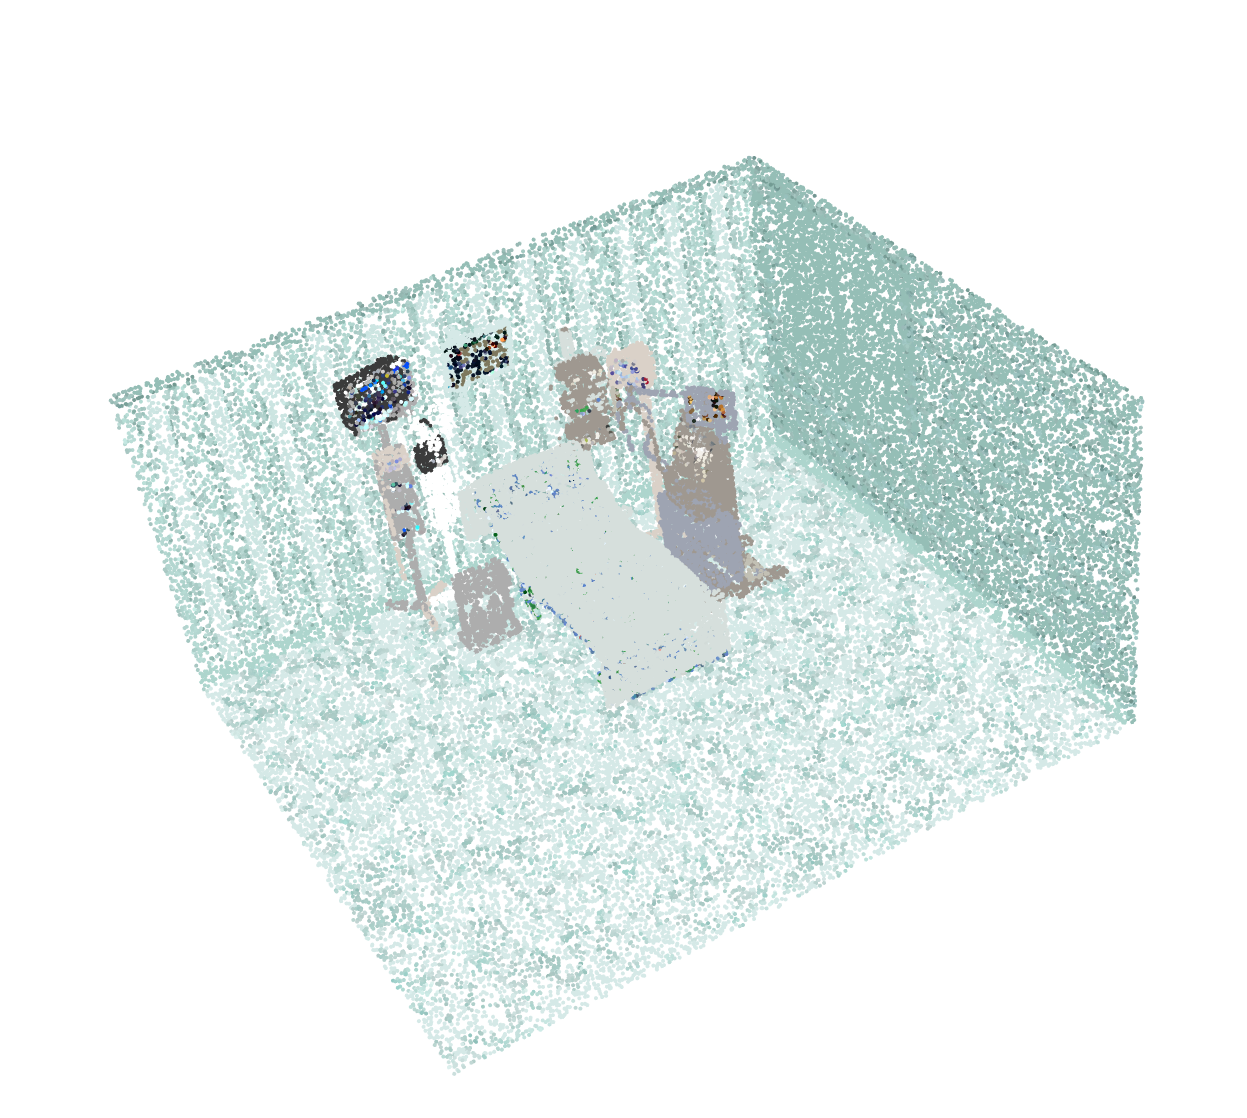
\includegraphics[width=0.49\columnwidth]{fig/icu_sampled.png}
    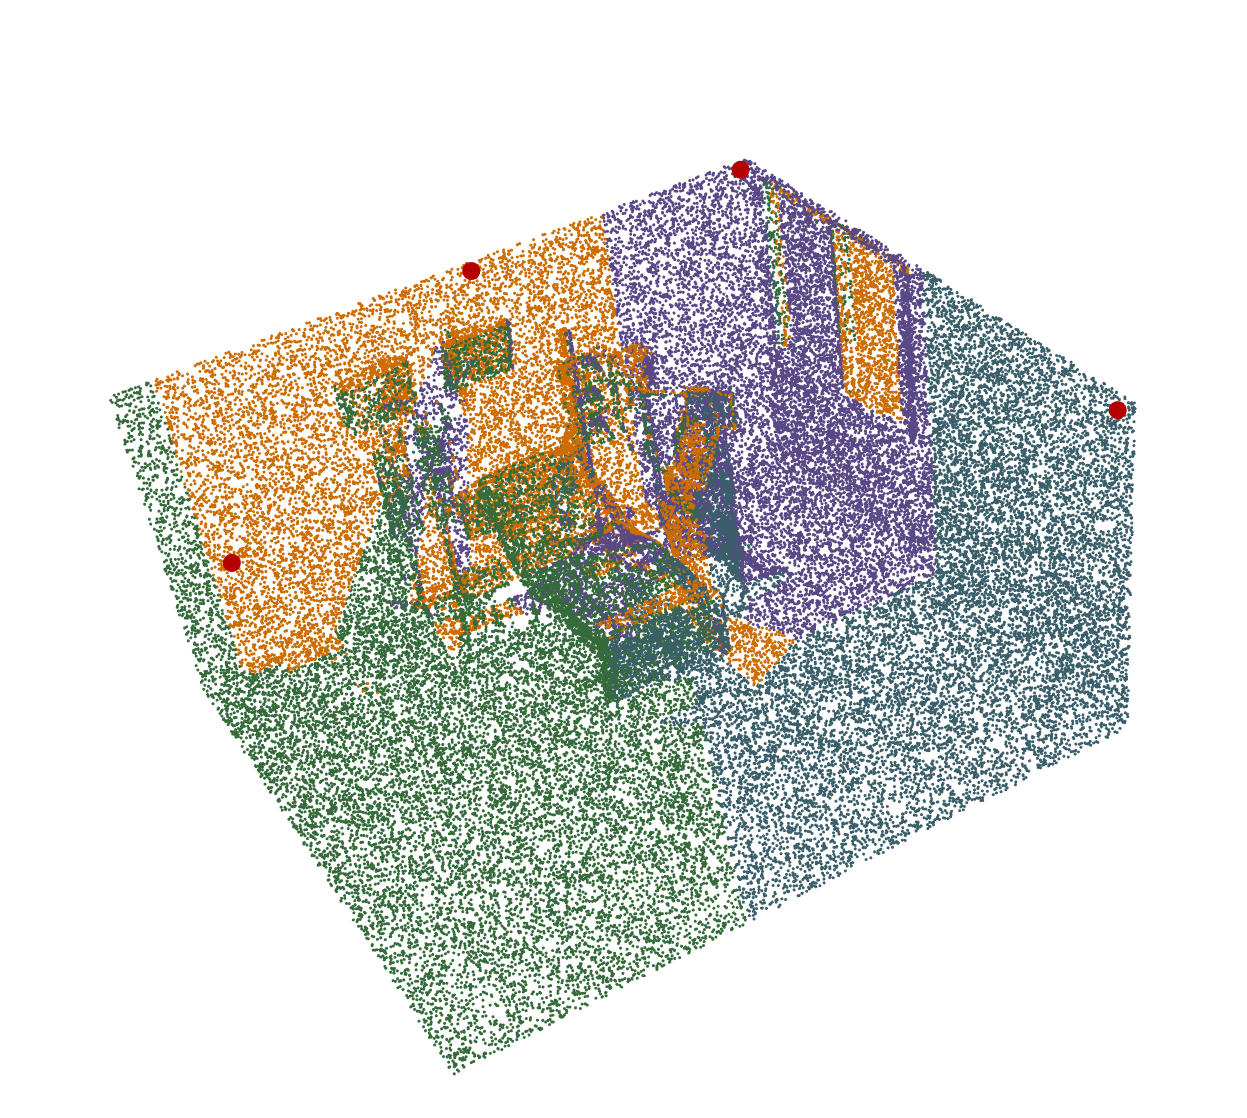
\includegraphics[width=0.49\columnwidth]{fig/icu_result.png}
    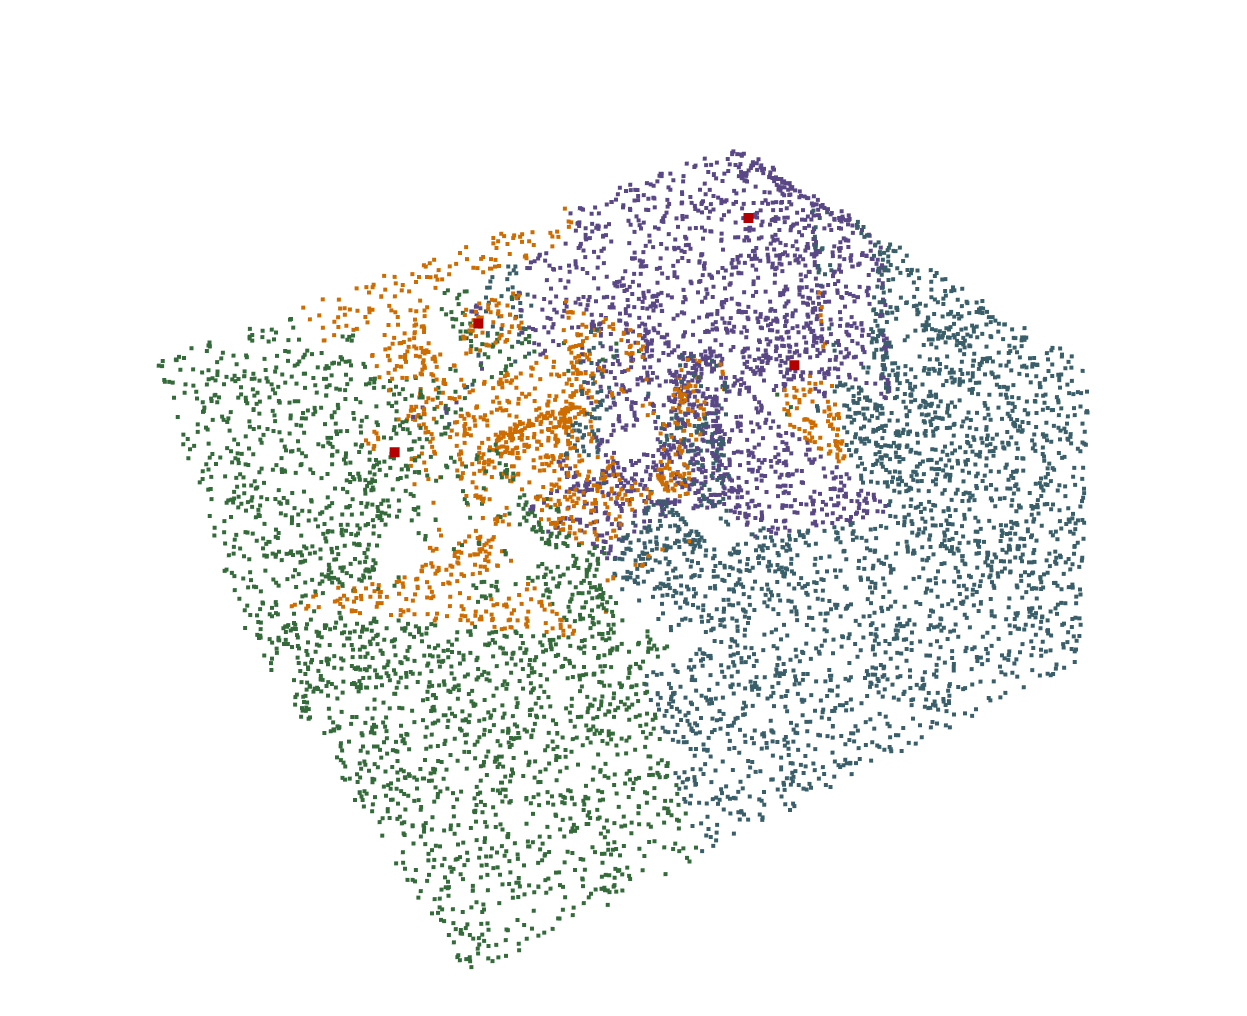
\includegraphics[width=0.49\columnwidth]{fig/icu_result_3.png}
    % 73965/ 78549
    
    % 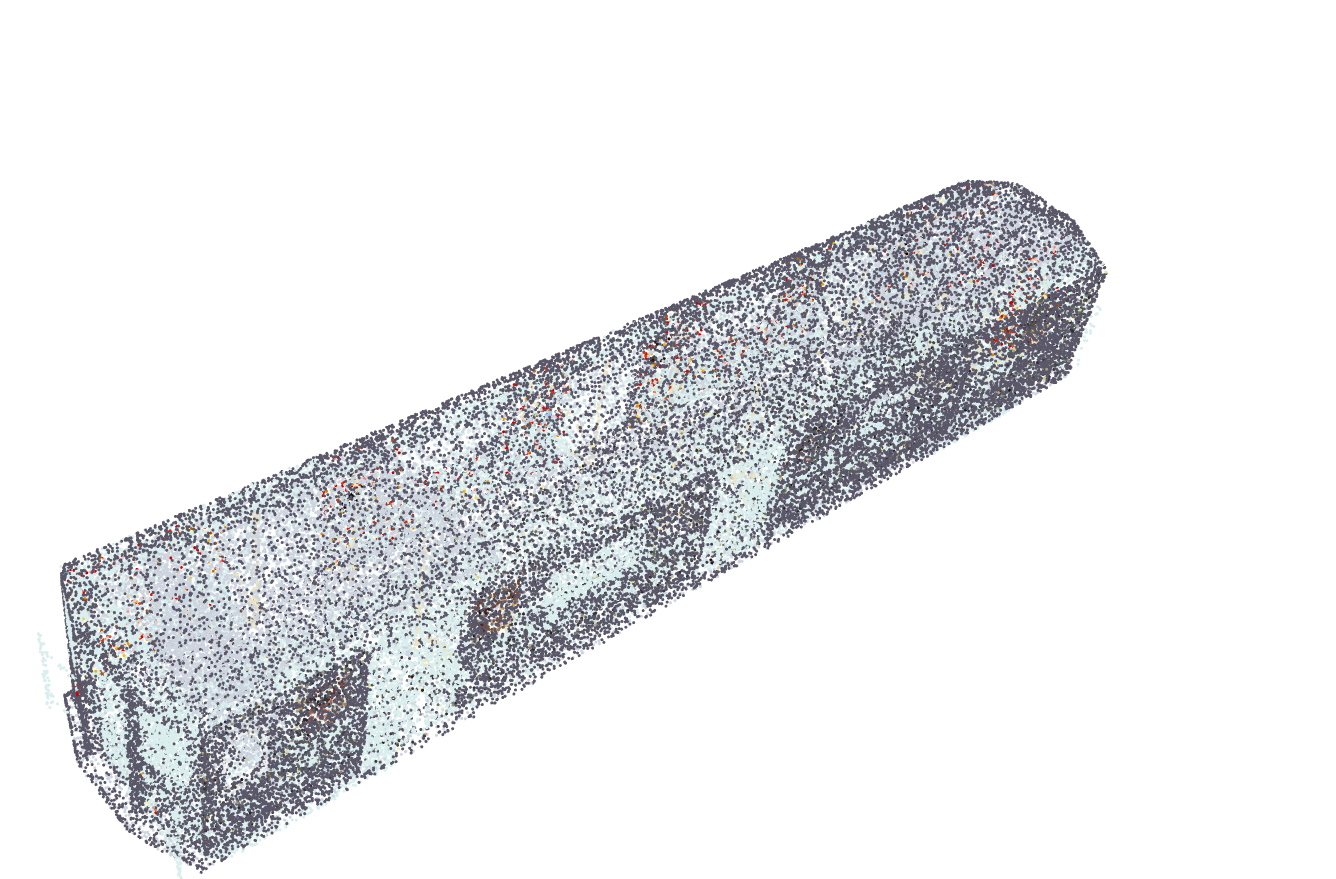
\includegraphics[width=0.52\columnwidth]{fig/train_sampled.png}
    \hspace{-0.1in}
    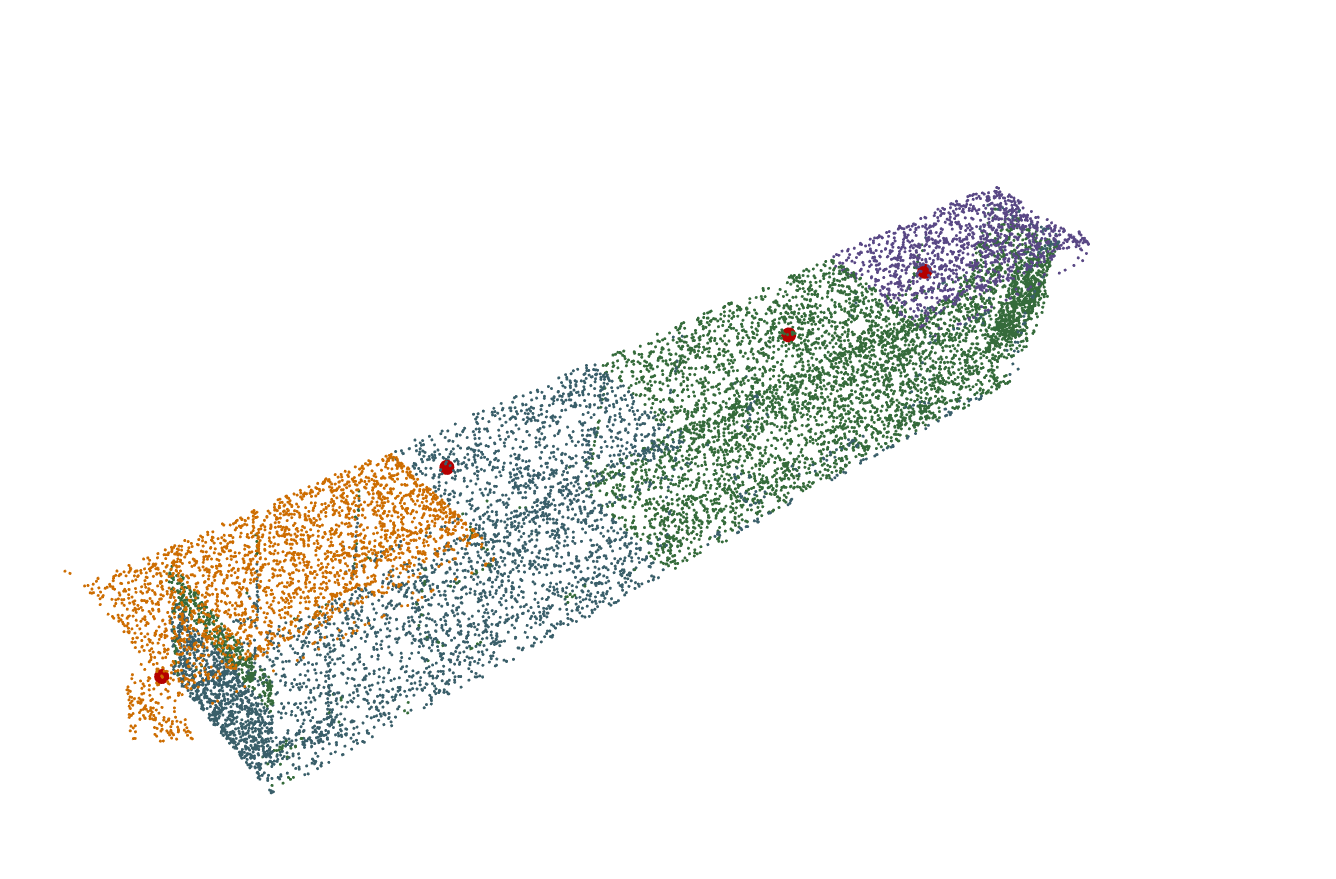
\includegraphics[width=0.54\columnwidth]{fig/train_result.png} 
    \hspace{-0.4in}
    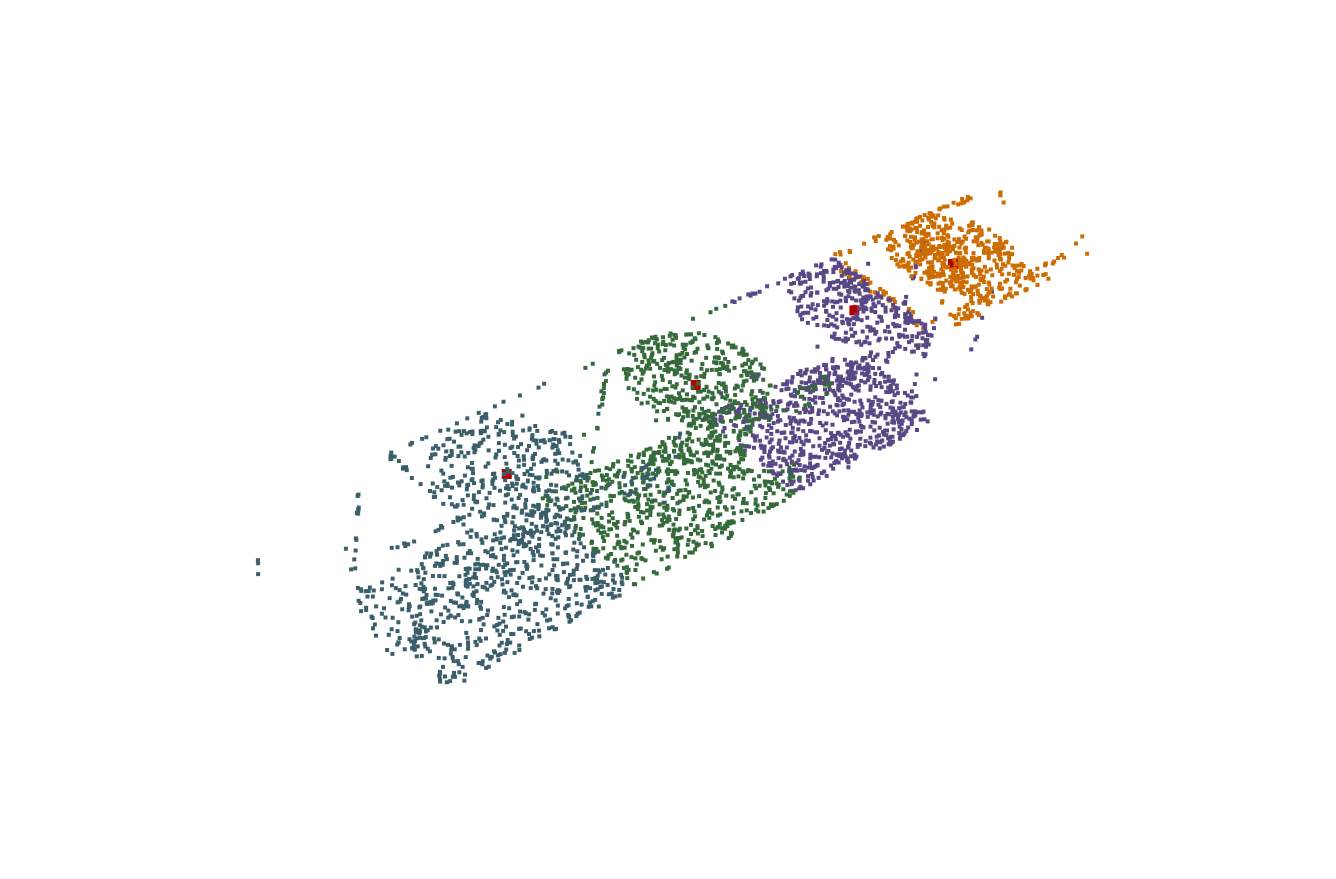
\includegraphics[width=0.54\columnwidth]{fig/train_result_3.png}
    % 14160 / 19604
    
    %\includegraphics[width=0.52\columnwidth]{fig/bus_original.png}
    % 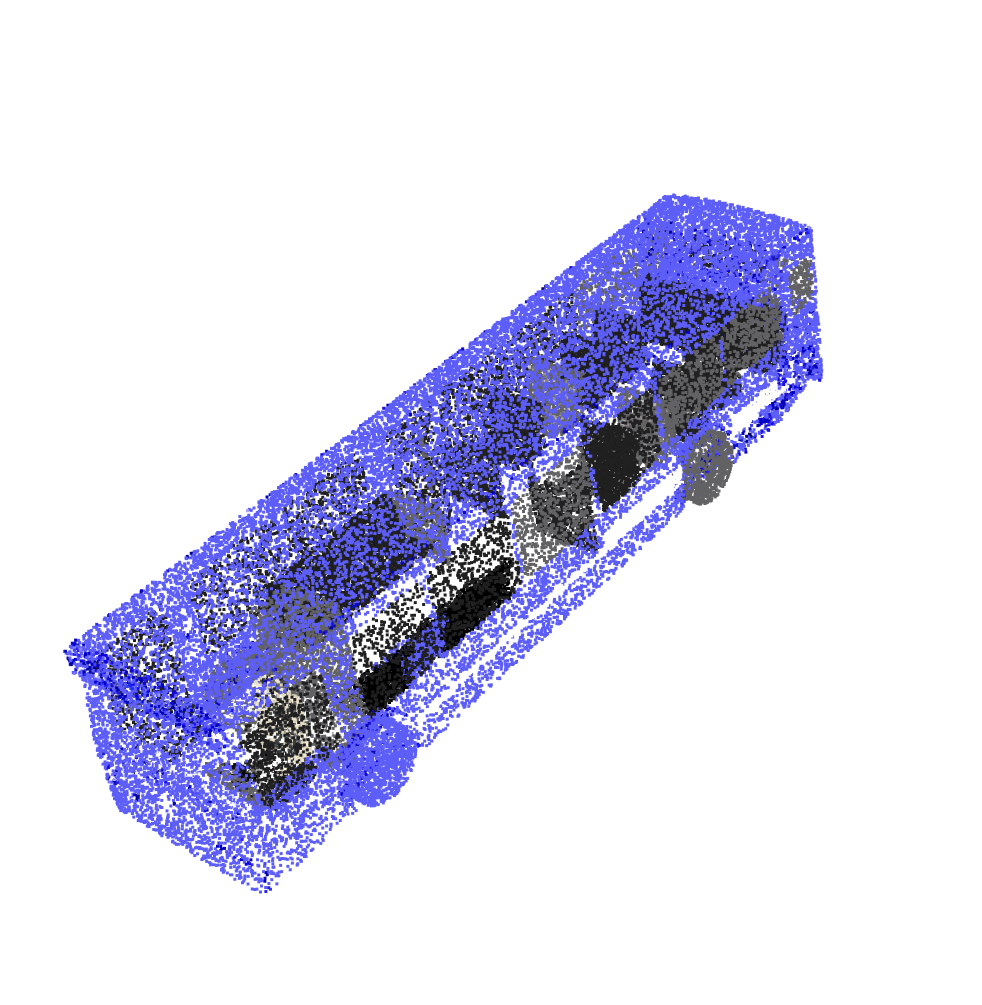
\includegraphics[width=0.52\columnwidth]{fig/bus_sampled.png}
    % \hspace{-0.3in}
    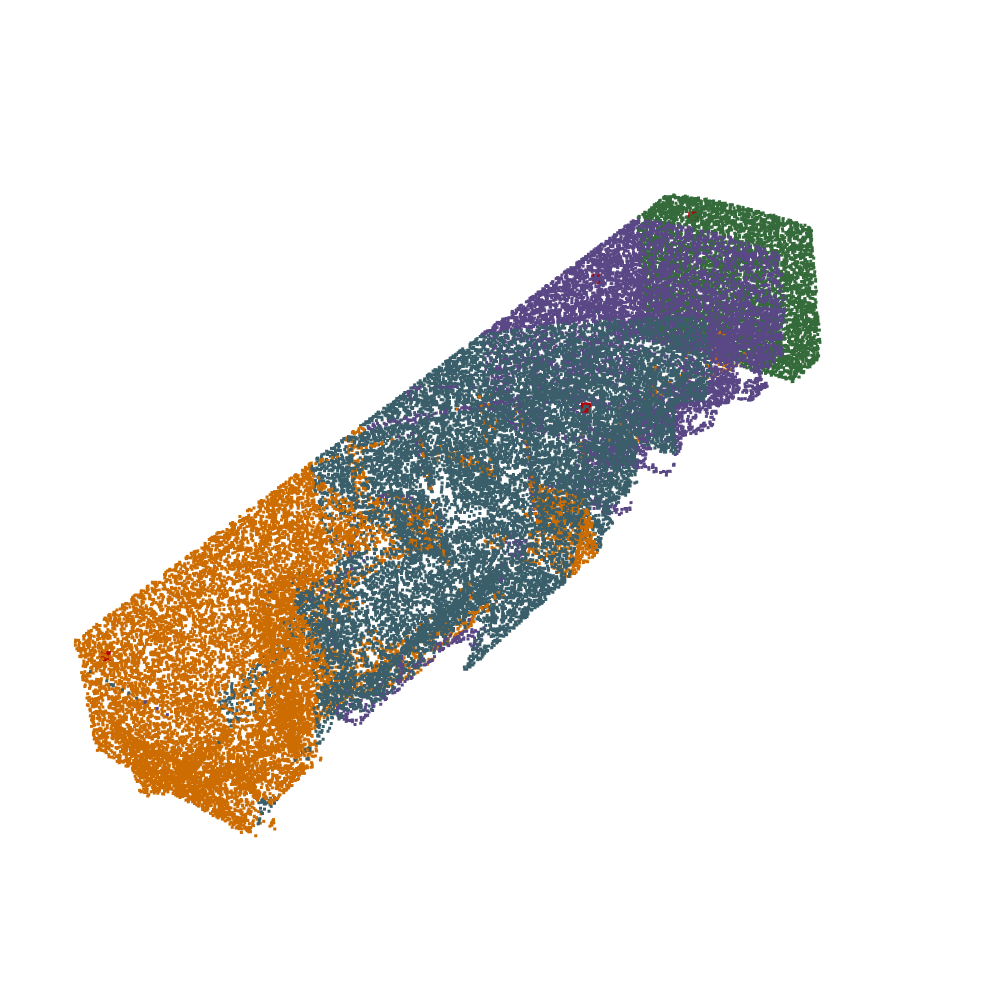
\includegraphics[width=0.52\columnwidth]{fig/bus_result.png} 
    \hspace{-0.3in}
    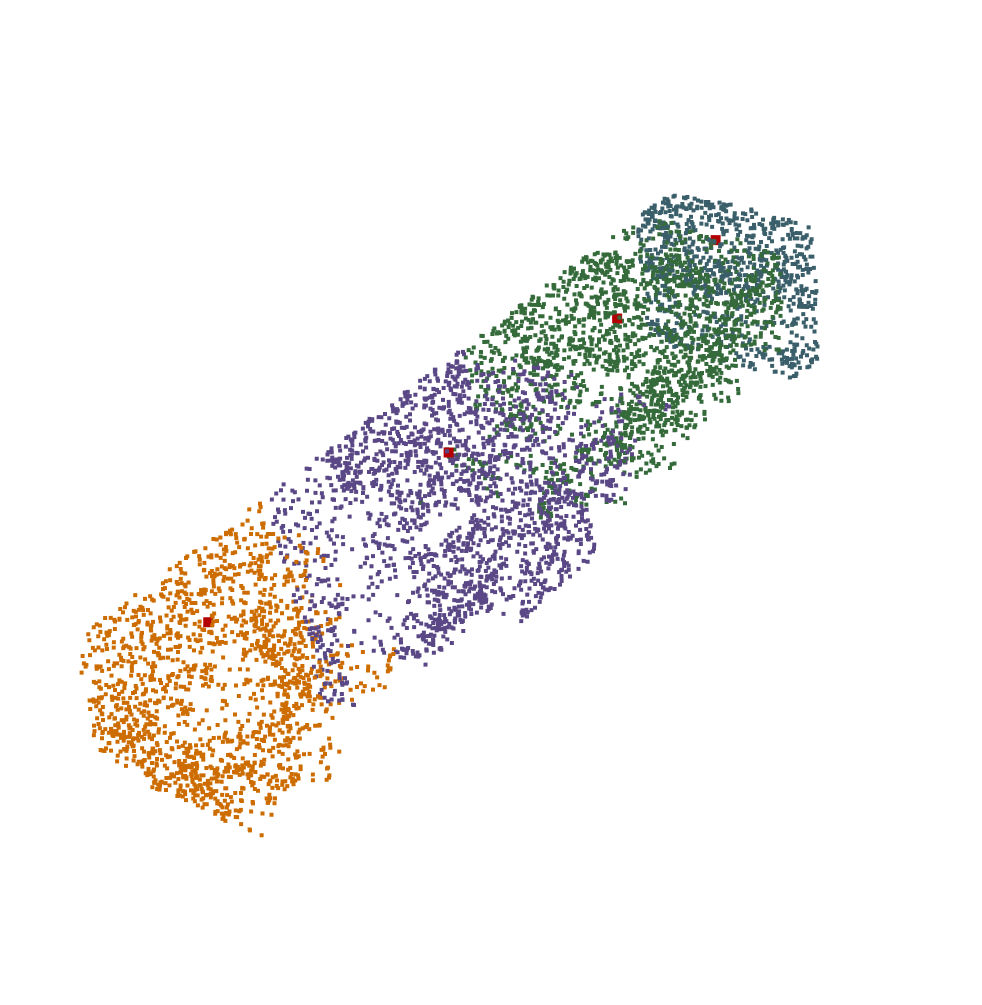
\includegraphics[width=0.52\columnwidth]{fig/bus_result_3.png} 
    % 45148 / 54229
    {
    \small{
    \caption{The illustration of the the results of coverage of the ICU, train and bus meshes using the visibility model and the cumulative exposure model using 4 sensors. 
    The coverage ratios are 94.2\%, 72.2\%, 83.2\%, for the visibility model, respectively. 
    The coverage ratios are 82.0\%, 38.6\%, 62.31\%, for the cumulative exposure model, respectively. 
    }
    }
    }
    \label{fig:my_label}
\end{figure}

\begin{figure}
    \centering
    \includegraphics[width = .31\columnwidth]{fig/illustration_bus.png}
    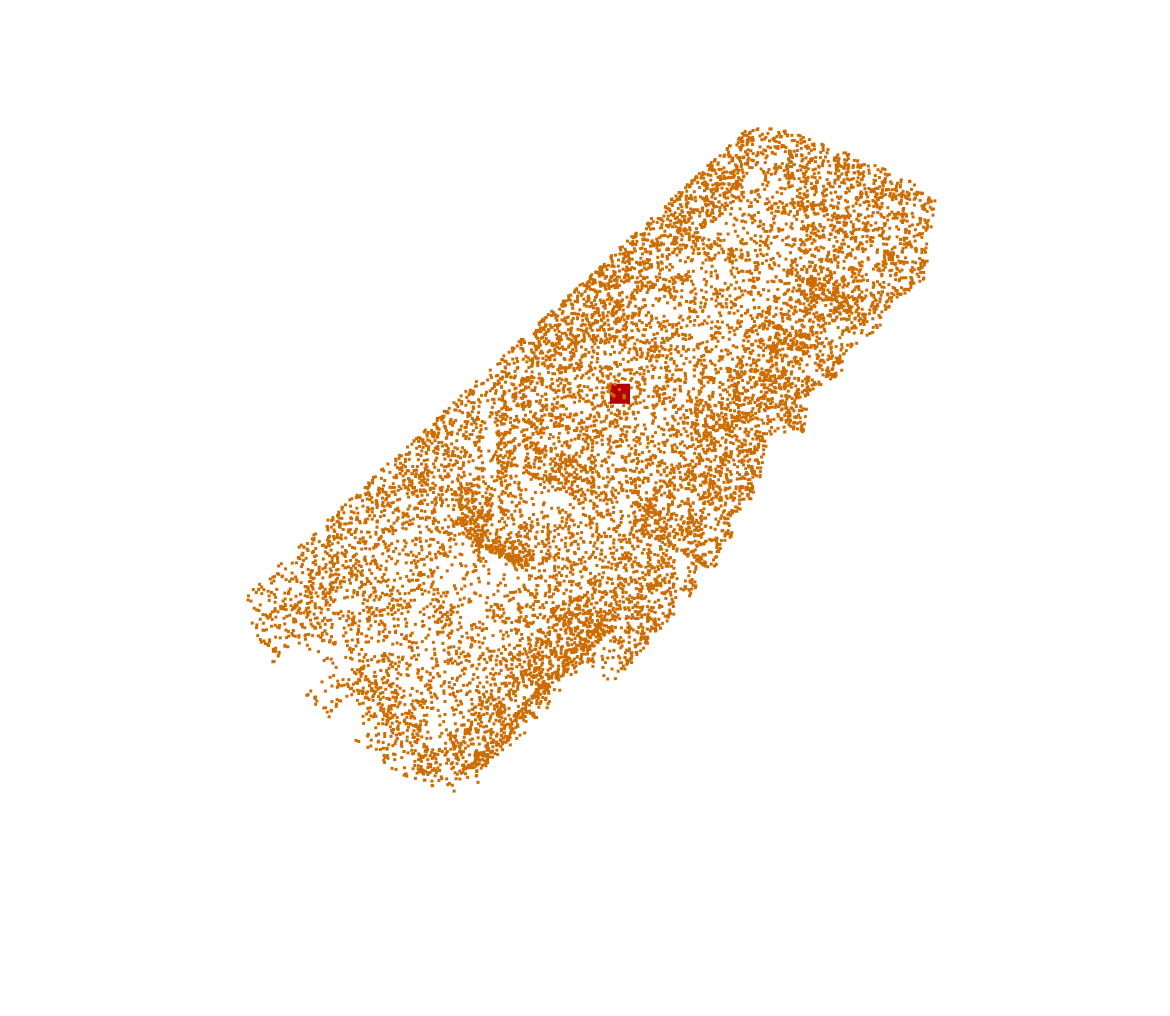
\includegraphics[width = .31\columnwidth]{fig/illustration_bus_mq_1.png}
    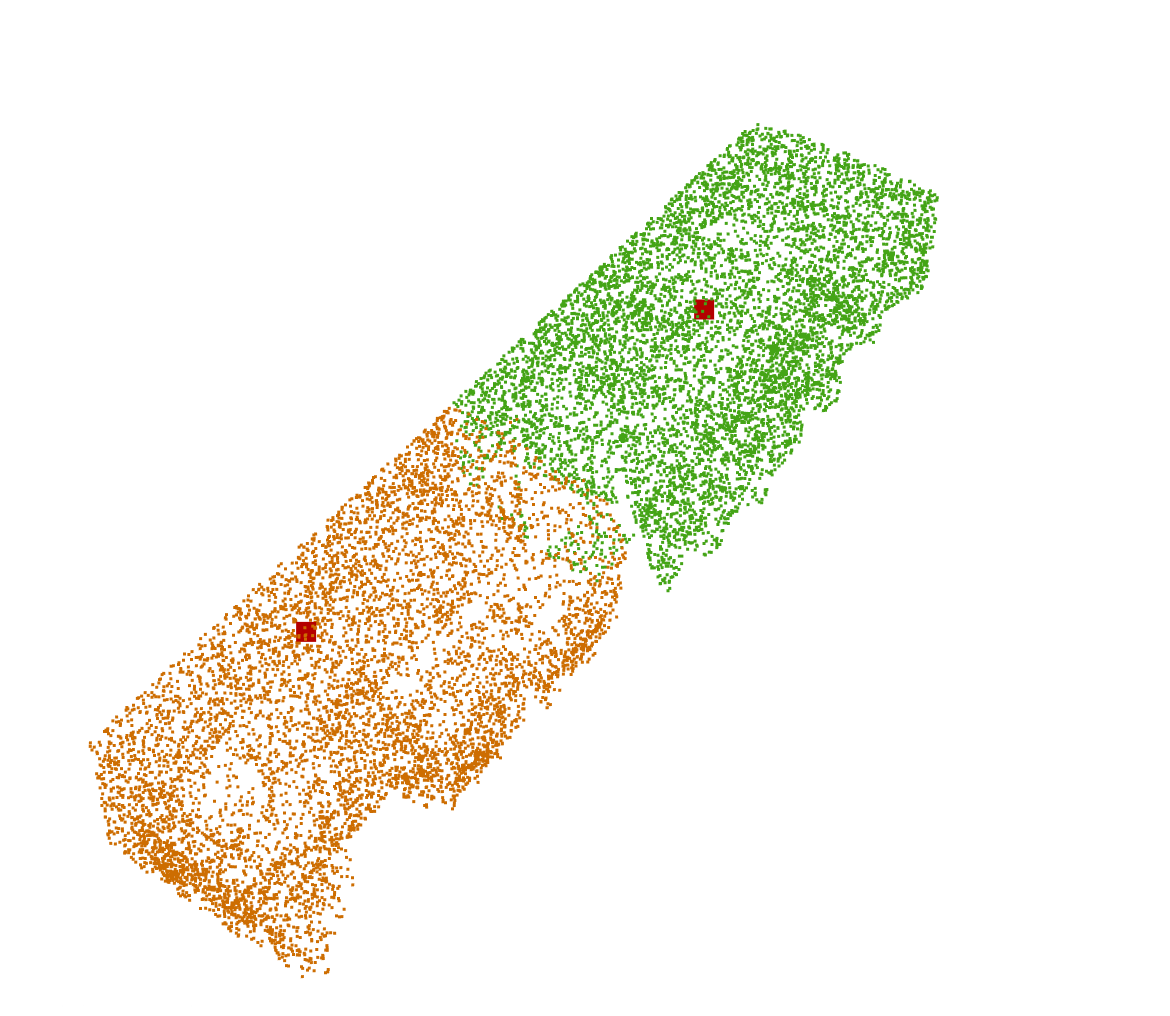
\includegraphics[width = .31\columnwidth]{fig/illustration_bus_mq_2.png}
    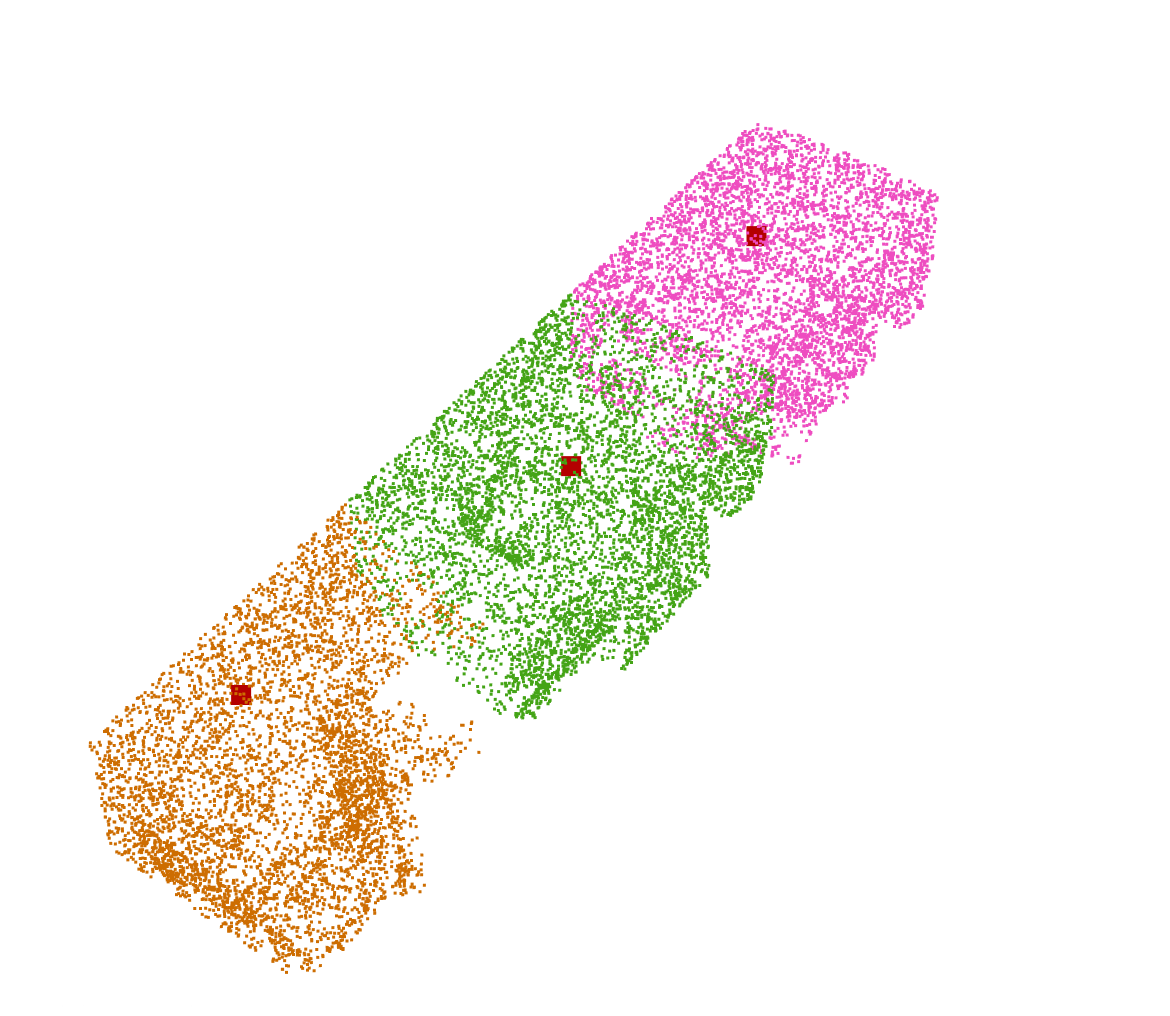
\includegraphics[width = .31\columnwidth]{fig/illustration_bus_mq_3.png}
    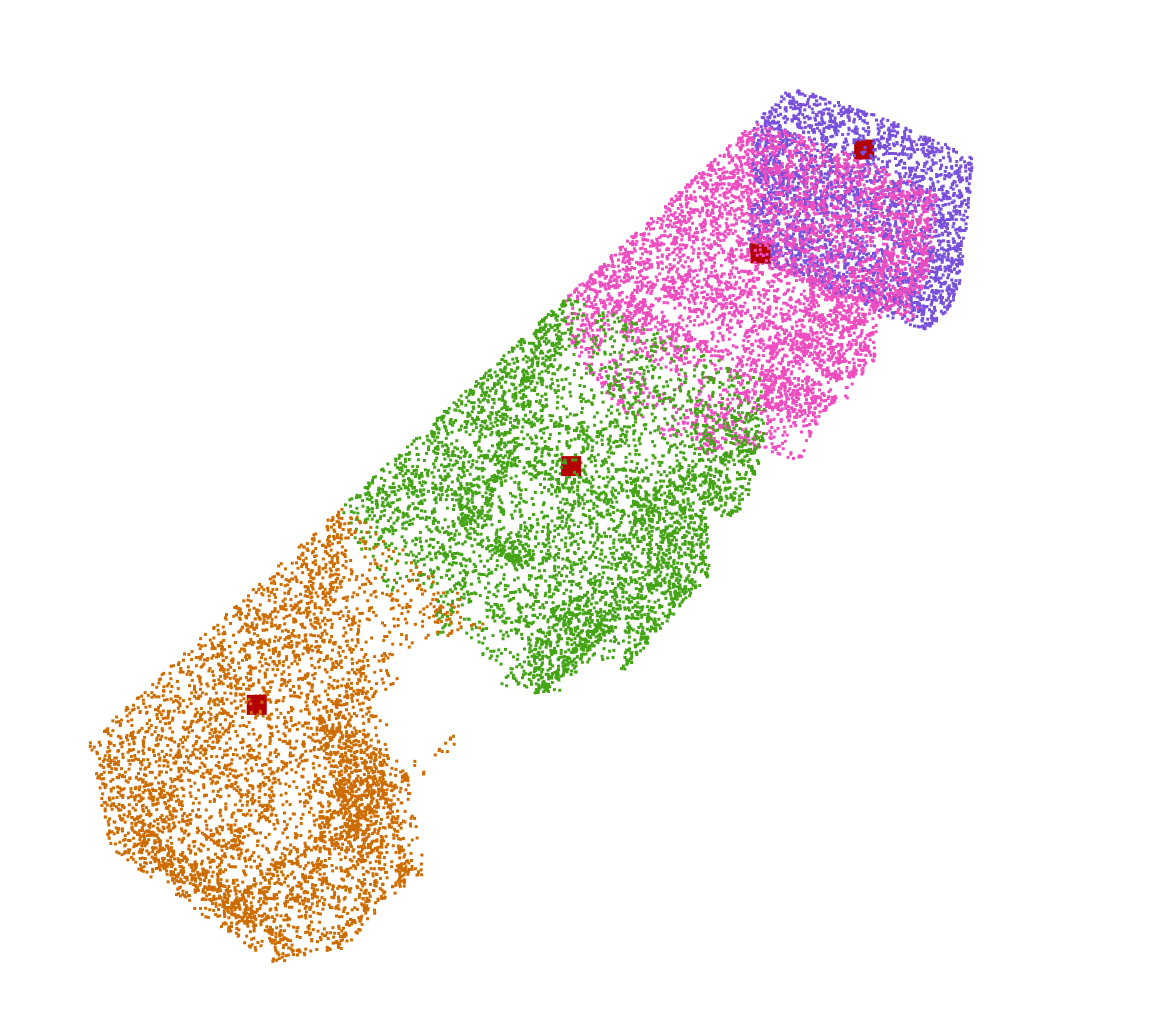
\includegraphics[width = .31\columnwidth]{fig/illustration_bus_mq_4.png}
    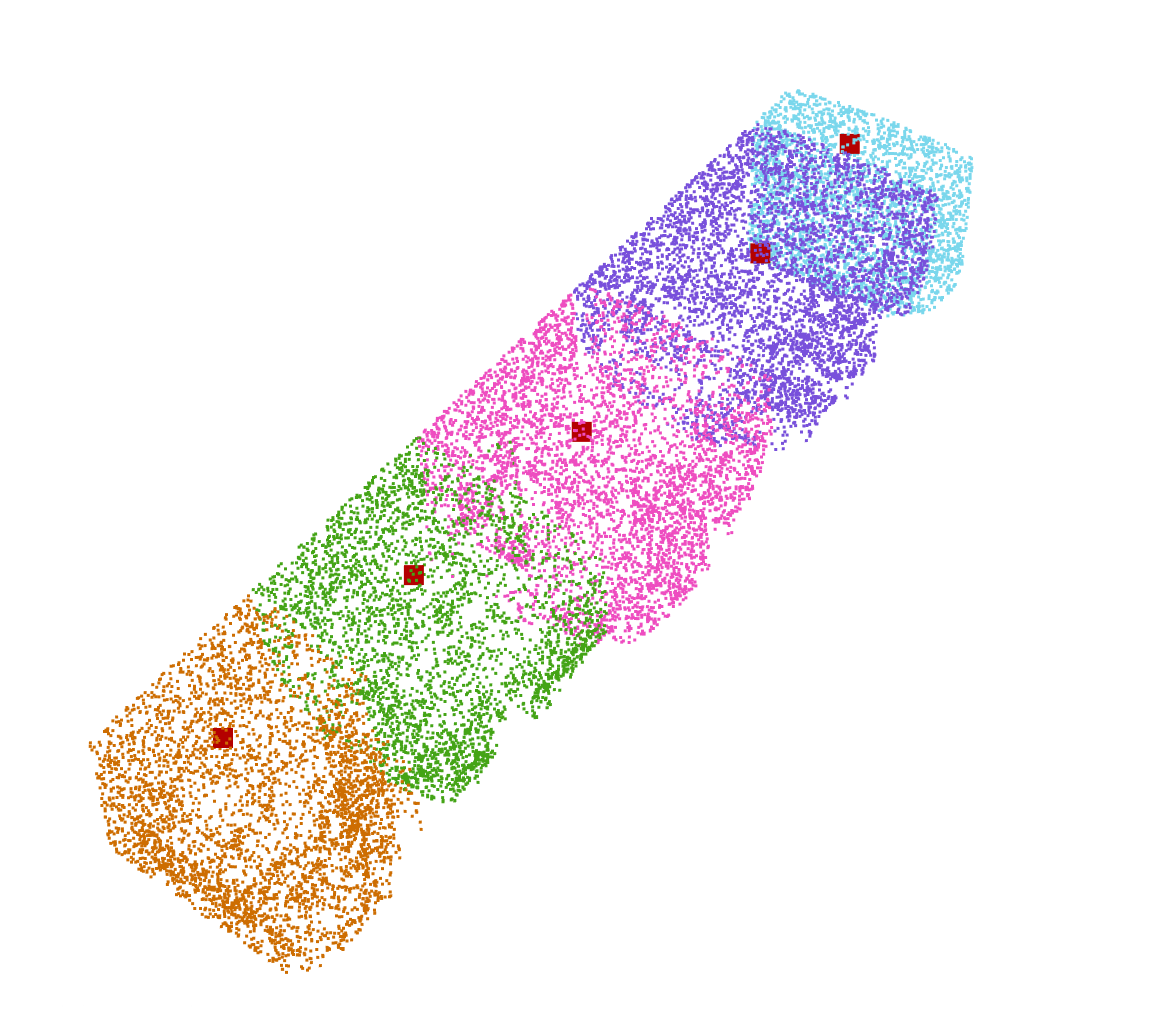
\includegraphics[width = .31\columnwidth]{fig/illustration_bus_mq_5.png}
    \caption{The coverage of the bus model using $1$ to $5$ lights with the maximum quality model.}
    \label{fig:my_label}
\end{figure}
\end{comment}

%% Comparison with different number of sensors problem 2


%% Comparison with different number of sensors
